\subsection{Trajectory Analysis}\label{sec:trajectory}

Though the completion time analysis indicates that Hydra / 3D headtracked
combination results in the fastest mean completion time, it possible to derive
insights from visualizing the data itself, in aggregate and on a per subject
basis.  These analyses are subjective.  In the following, all input data were
normalized so that the start target is at the origin and the end target lies
on the positive $x$-axis.

\figref{fig:compressedtracks} shows the tracks for each input/output
combination. Each path is data from a trial; green indicates a trial
completion time of less than 10 seconds and red is over 10 seconds.  Each
point was rotated around the $x$-axis so that it lies on the XY plane,
discarding Z information while minimizing angular distortion.

\begin{figure}
    \centering
    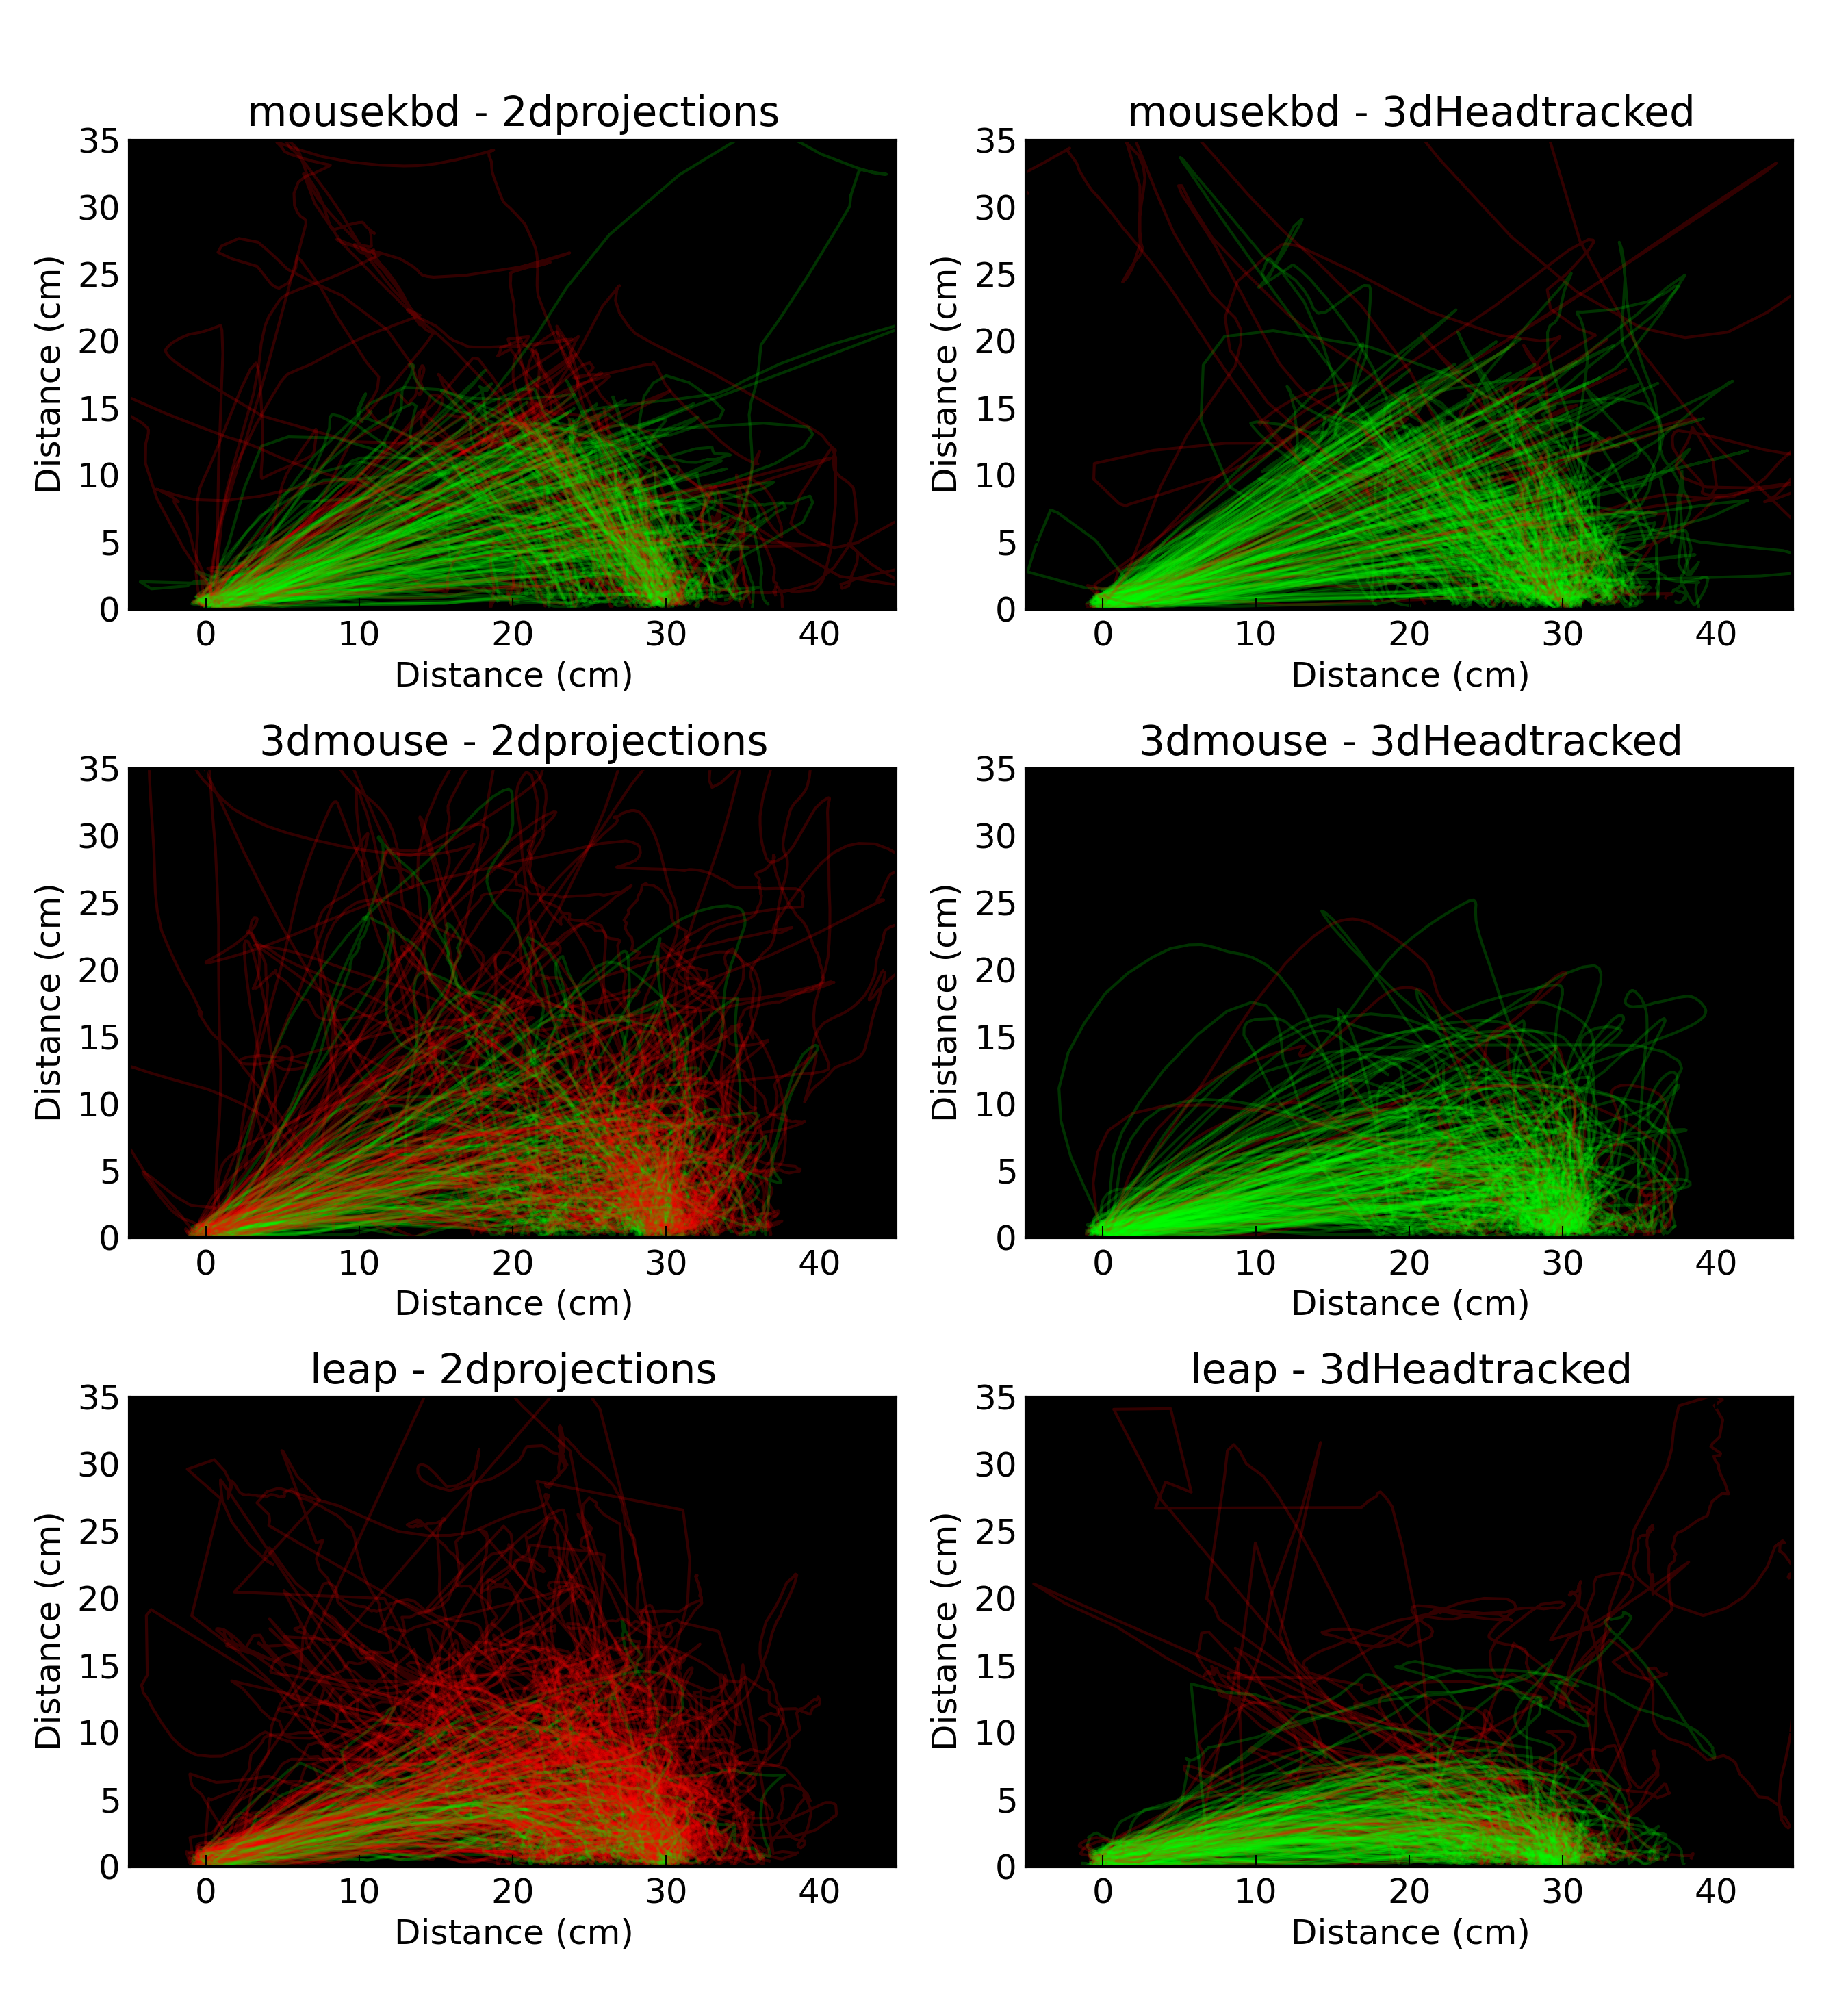
\includegraphics[width=\columnwidth]{paths.png}
    \caption{Cylinder compressed tracks}
    \label{fig:compressedtracks}
\end{figure}

We can see that subjects adopted similar strategies for the mouse and keyboard
regardless of the display type: straight line movements in orthogonal planes.
Orthogonality can't be avoided, but this shows that skills developed in
traditional 2D displays readily transfer.  That is, though the mouse is a
relative positioning input device, users have good mouse-eye coordination that
allows them to quickly reposition the cursor on a plane using mostly straight
line motions.

The straight-line orthogonal movement strategy is also somewhat evident for
the 3D mouse and Leap in the 2D projection case, but their tracks are more
organic looking.  From observing the subjects we noticed that, especially for
the 3D mouse, 3D inputs in the 2D projection case were unintuitive for most
subjects, but that after even the 20 trials conducted, they were able to learn
a decent mapping from hand motion to cursor motion.  See for example
\figref{fig:improvementtimes}.

\figref{fig:improvementtimes} which shows the average reduction in completion
time between the first 3 trials of 20 for an input/output combination, and the
last 3.  We interpret a small reduction as meaning not much learning had to or
could take place to saturate proficiency (median close to zero), whereas a
large reduction (median far from zero) is indicative of an \emph{unintuitive}
input modality.  For example, subjects did not tend to get much better using
the mouse and keyboard, irrespective of output type (saturated prior
experience), nor on the Leap in the 3D headtracked case (intuitive), but they
did improve quite a bit on the 3D mouse in the 2D projections case
(unintuitive).  Note that positive times are partially due to noise induced by
the random target positioning

\begin{figure}
    \centering
    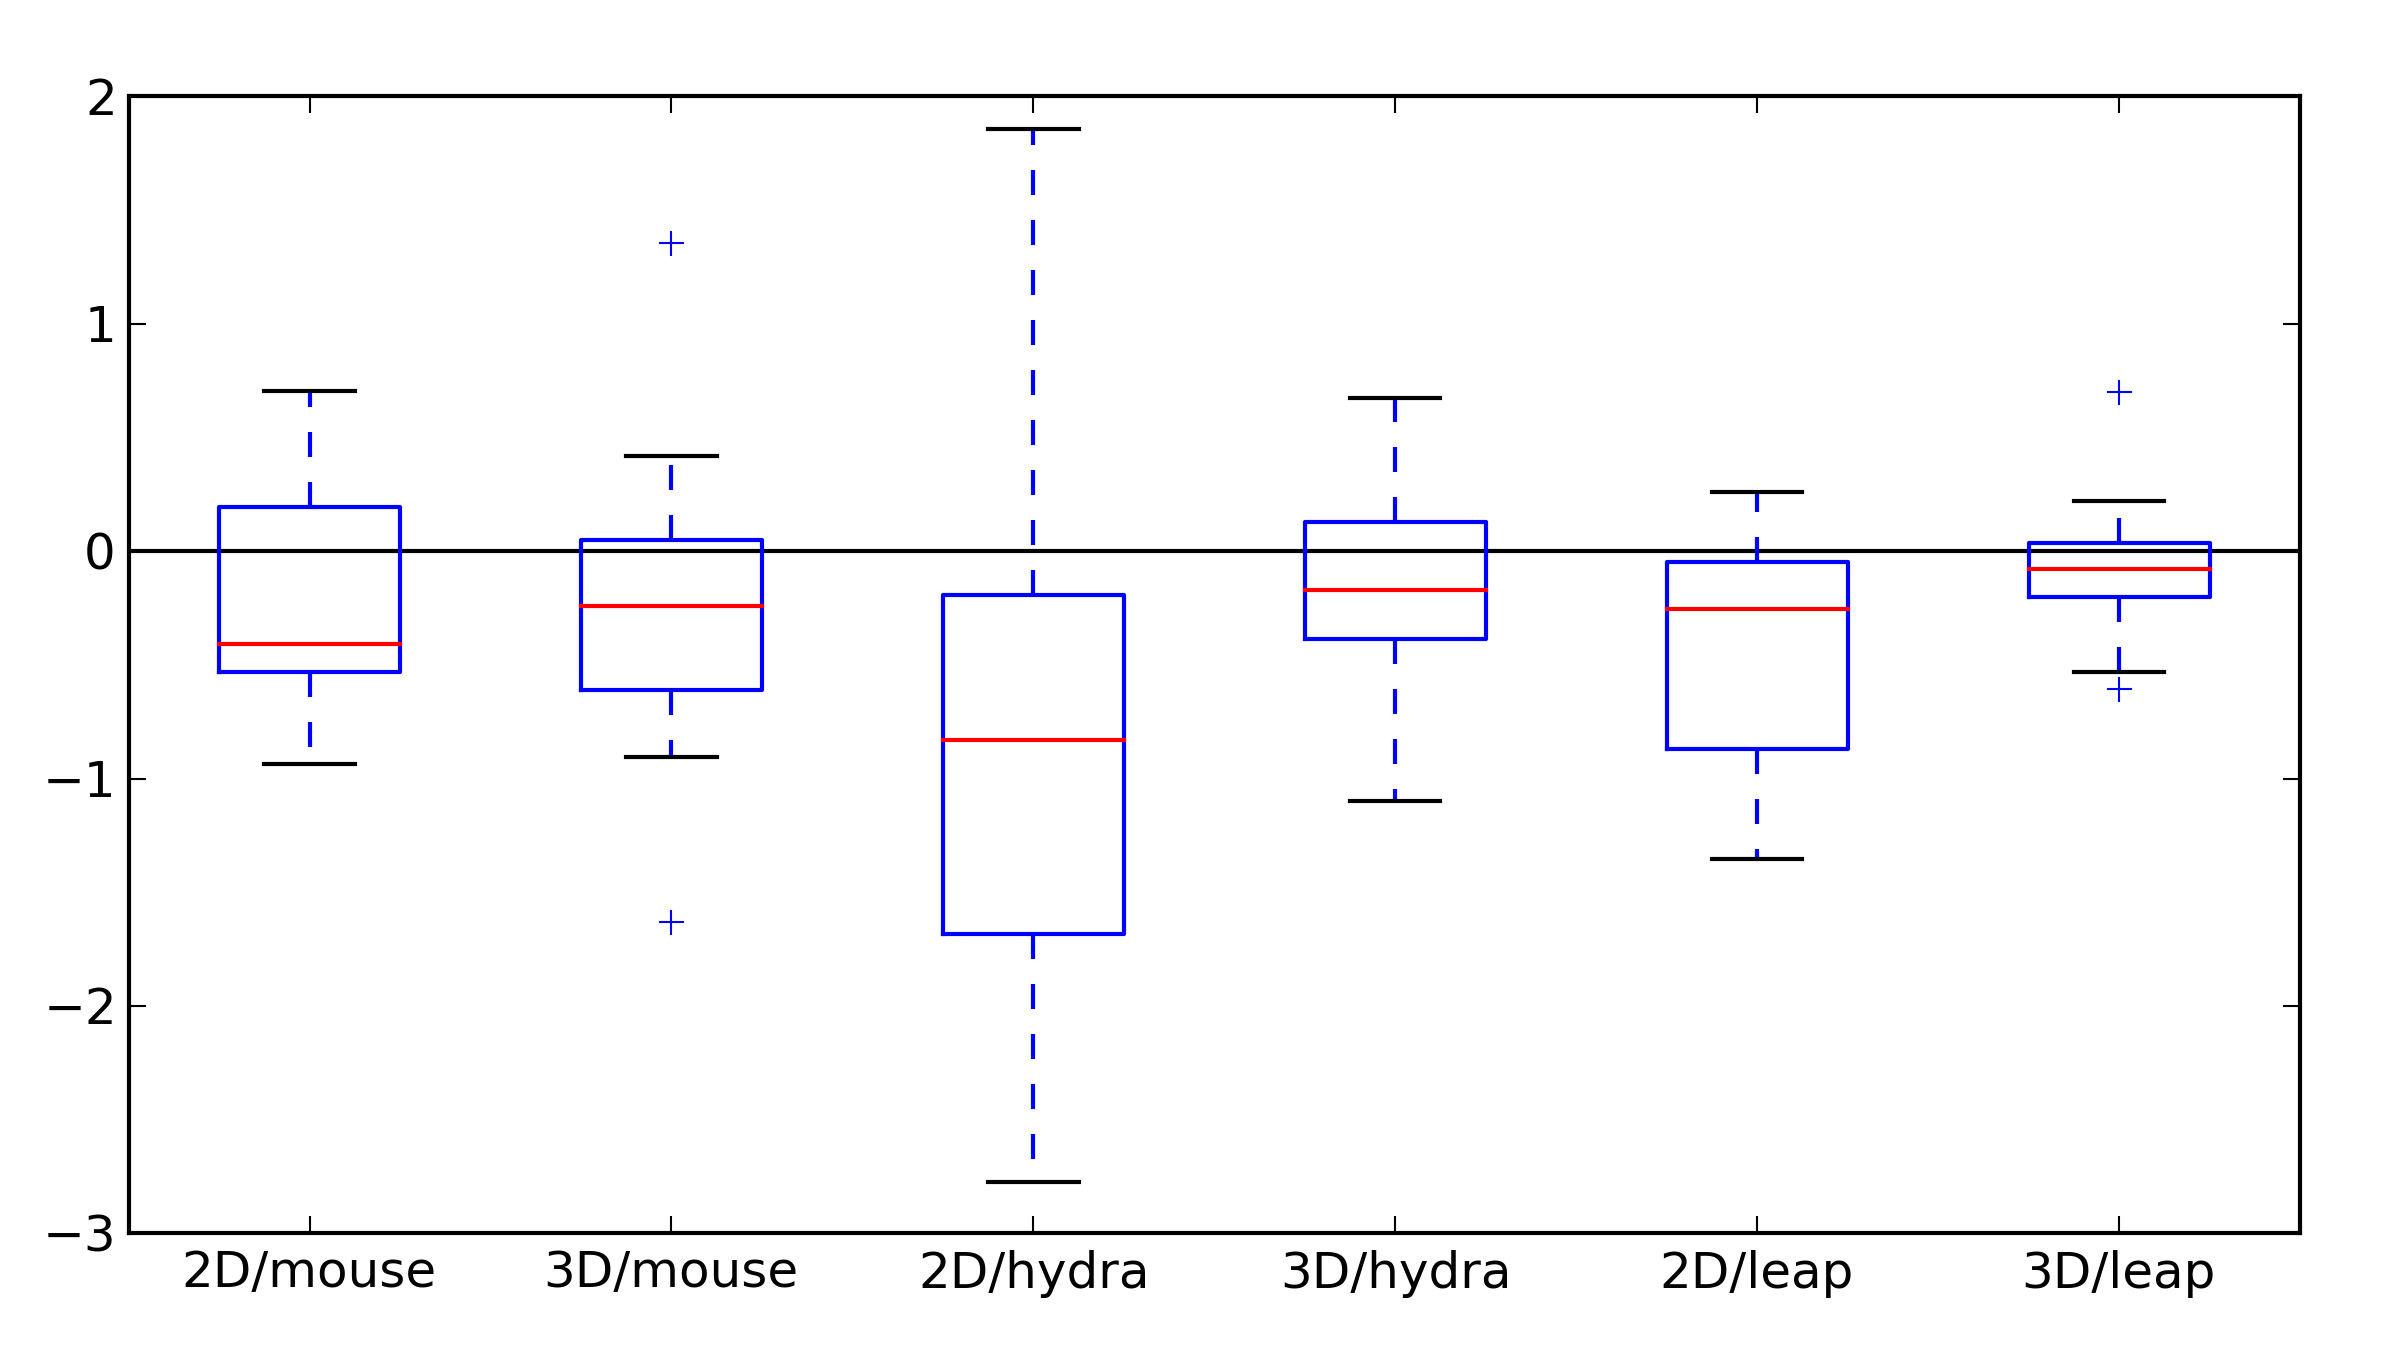
\includegraphics[width=\columnwidth]{improvement.png}
    \caption{Learning the inputs, reduction in completion time (s).}
    \label{fig:improvementtimes}
\end{figure}

\figref{fig:deviation} plots the average perpendicular distance (deviation) from
the start-end target line segment for each subject for each input/output
modality.  A deviation of 0 would mean the cursor moved on a perfectly
straight path between the two targts.  We see there is significant inter
subject variance for the deviation, almost independent of input type.  For
example, subject 12 had the largest deviation for the mouse and keyboard / 2D
projections case, but one of the smaller for Leap / 3D headtracked.  The large
deviations in the Leap/ 3D headtracked case are mostly due to the Leap not
working correctly.

From the standpoint of adopting a new system in an organization,
\figref{fig:deviation} would indicate that some people will need extra time to
accustom themselves.  This extra time for familiarization should be taken into
account, e.g. by cautioning against getting frustrated right away.

\begin{figure}
  \centering
  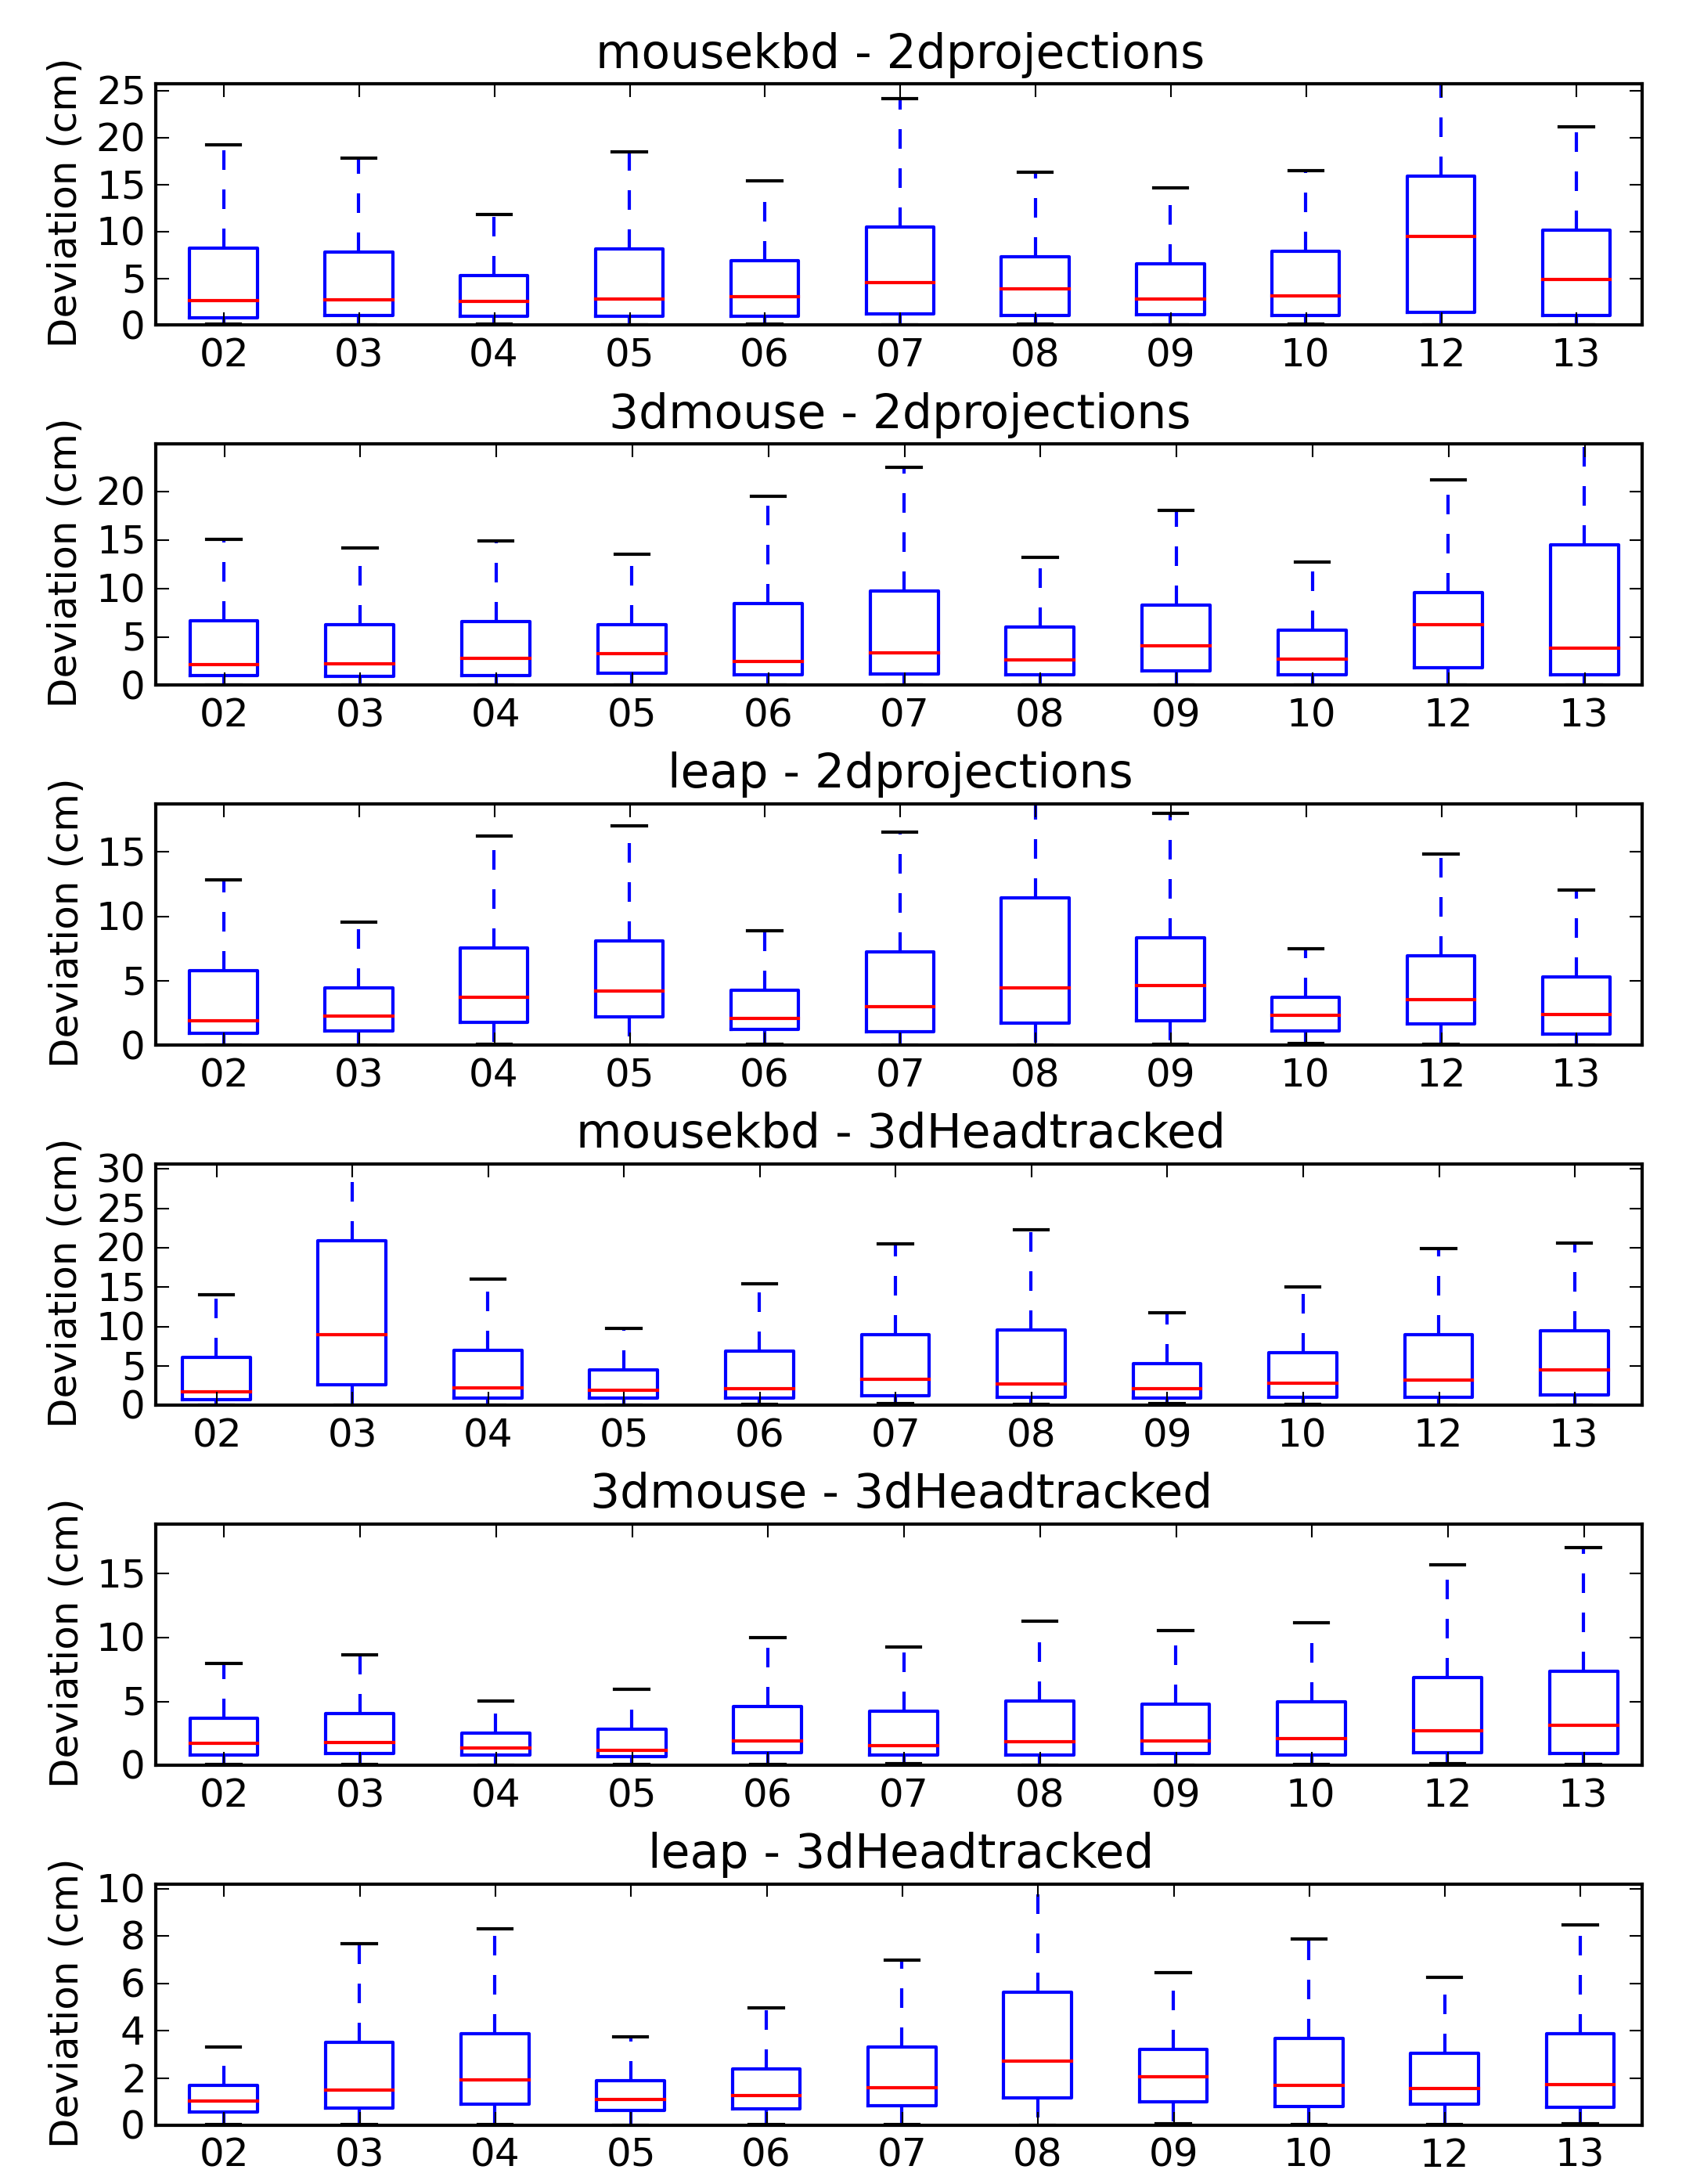
\includegraphics[width=\columnwidth]{deviation.png}
  \caption{Mean perpendicular distance from start-end line segment}
  \label{fig:deviation}
\end{figure}

